\documentclass[aspectratio=169, table]{beamer}

\usepackage{listings}
\usepackage{tikz}
\usetikzlibrary{positioning, arrows.meta, fit}



\lstdefinestyle{RustStyle}{
	language=Java,
	morekeywords={println, Ok, async, fn, main, use, let, mut},
	basicstyle=\ttfamily\scriptsize,
	keywordstyle=\color{blue},
	commentstyle=\color{gray},
	stringstyle=\color{red},
	breaklines=true,
	showstringspaces=false,
	tabsize=2,
	captionpos=b,
	numbers=left,
	numberstyle=\tiny\color{gray},
	frame=lines,
	backgroundcolor=\color{lightgray!10},
	comment=[l]{//},
	morecomment=[s]{/*}{*/},
	commentstyle=\color{gray}\ttfamily,
	string=[s]{'}{'},
	morestring=[s]{"}{"},
	stringstyle=\color{teal}\ttfamily,
	%	showstringspaces=false
	literate=
	{\{}{{\textcolor{red}{\{}}}1
	{\}}{{\textcolor{red}{\}}}}1
	{:}{{\textcolor{red}{:}}}1
	{=}{{\textcolor{red}{=}}}1
	{.}{{\textcolor{red}{.}}}1
	{]}{{\textcolor{red}{]}}}1
	{[}{{\textcolor{red}{[}}}1
	{\#}{{\textcolor{red}{\#}}}1
	{;}{{\textcolor{red}{;}}}1
	{?}{{\textcolor{red}{?}}}1
	{!}{{\textcolor{red}{!}}}1
}

%\usepackage[beamertheme=./praditatheme]{Pradita}

\usetheme{Pradita}

\lstdefinelanguage{bash} {
	keywords={},
	basicstyle=\ttfamily\small,
	keywordstyle=\color{blue}\bfseries,
	ndkeywords={iex},
	ndkeywordstyle=\color{purple}\bfseries,
	sensitive=true,
	commentstyle=\color{gray},
	stringstyle=\color{red},
	numbers=left,
	numberstyle=\tiny\color{gray},
	breaklines=true,
	frame=lines,
	backgroundcolor=\color{lightgray!10},
	tabsize=2,
	comment=[l]{\#},
	morecomment=[s]{/*}{*/},
	commentstyle=\color{gray}\ttfamily,
	stringstyle=\color{purple}\ttfamily,
	showstringspaces=false
}


\title{\Huge Event-Driven\\Architecture\\}
\subtitle{IF231303-Software Architecture}
\author{\textbf{Alfa Yohannis}}
\begin{document}
	
	\frame{\titlepage}
	
	
	\begin{frame}[fragile]
		\frametitle{Contents}
		\vspace{20pt}
		\begin{columns}[t]
			\column{0.5\textwidth}
			\tableofcontents[sections={1-5}]
			
			\column{0.5\textwidth}
			\tableofcontents[sections={6-10}]
		\end{columns}
	\end{frame}
		
	\section{Introduction}
	
	\begin{frame}[fragile]{Event-Driven Architecture (EDA)}
		\vspace{20pt}
		\begin{columns}[T]
			\column{0.5\textwidth}
			\textbf{Definition:}
			\begin{itemize}
				\item Focuses on producing, detecting, consuming, and reacting to events
				\item Systems driven by event-triggered data flow and logic
				\item Loose coupling between components
			\end{itemize}
			
			\textbf{When to Use:}
			\begin{itemize}
				\item Real-time response needs
				\item Unpredictable workloads
				\item Distributed applications
			\end{itemize}
			
			\column{0.5\textwidth}
			\textbf{Key Benefits:}
			\begin{itemize}
				\item Reactive and flexible systems
				\item Adaptable to environment changes
				\item Scalable and resilient
			\end{itemize}
			
			\textbf{Examples:}
			\begin{itemize}
				\item Financial transaction processing
				\item IoT sensor monitoring
				\item Microservices integration
				\item Notification platforms
			\end{itemize}
		\end{columns}
	\end{frame}
	
	\section{Use Case Examples}
	
	\begin{frame}[fragile]{Use Cases}
		\vspace{20pt}
		\begin{columns}[T]
			\column{0.33\textwidth}
			\textbf{Real-Time Monitoring}
			\begin{itemize}
				\item Track status and data changes instantly
				\item Example: Industrial machine sensors (temperature, vibration)
				\item Benefits:
				\begin{itemize}
					\item Immediate alarms and analysis
					\item No need for polling
				\end{itemize}
			\end{itemize}
			
			\column{0.33\textwidth}
			\textbf{System Integration}
			\begin{itemize}
				\item Connect independent systems via events
				\item Example: "PaymentCompleted" triggers inventory and shipping
				\item Benefits:
				\begin{itemize}
					\item Loose coupling
					\item Asynchronous, scalable communication
				\end{itemize}
			\end{itemize}
			
			\column{0.33\textwidth}
			\textbf{Microservices Architecture}
			\begin{itemize}
				\item Services act as event producers and consumers
				\item Example: "OrderCreated" event consumed by multiple services
				\item Benefits:
				\begin{itemize}
					\item Modular and resilient
					\item Easier scaling and deployment
				\end{itemize}
			\end{itemize}
		\end{columns}
	\end{frame}
	
	
	\section{Strengths and Limitations}
	
	\begin{frame}[fragile]{Strengths and Limitations}
		\vspace{10pt}
		\begin{columns}[T]
			\column{0.5\textwidth}
			\textbf{Strengths}
			\begin{itemize}
				\item \textbf{Loose Coupling:} Components evolve independently
				\item \textbf{High Scalability:} Events processed in parallel
				\item \textbf{Real-Time Responsiveness:} Immediate reactions without polling
				\item \textbf{Flexible Integration:} Easy cross-system communication
				\item \textbf{Modular Development:} Faster, isolated deployments
			\end{itemize}
			
			\column{0.5\textwidth}
			\textbf{Limitations}
			\begin{itemize}
				\item \textbf{Harder Debugging/Tracing:} Complex event flows
				\item \textbf{Data Consistency Challenges:} Distributed transaction risks
				\item \textbf{Infrastructure Complexity:} Requires robust messaging backbone
				\item \textbf{Error and Duplication Handling:} Retry, idempotency needed
				\item \textbf{Learning Curve:} Extra skills and patterns required
			\end{itemize}
		\end{columns}
	\end{frame}
	
	\section{Core Concepts}
	
	\begin{frame}{Core Concepts of EDA Flow}
		\vspace{10pt}
		\centering
		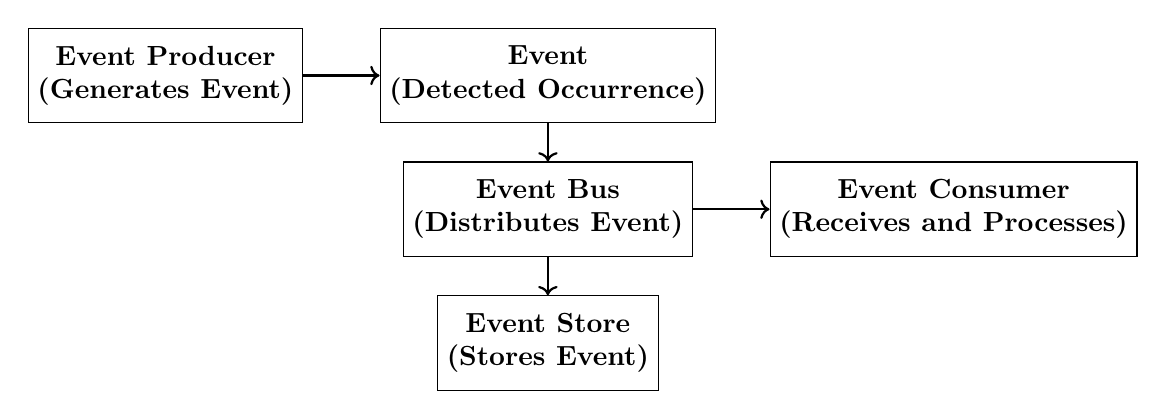
\begin{tikzpicture}[
			node distance=0.04\textwidth and 0.08\textwidth,
			every node/.style={draw, align=center, minimum height=1.2cm, minimum width=0.18\textwidth, font=\bfseries},
			arrow/.style={->, thick}
			]
			% Nodes
			\node (producer) {Event Producer \\ (Generates Event)};
			\node (event) [right=of producer] {Event \\ (Detected Occurrence)};
			\node (bus) [below=of event] {Event Bus \\ (Distributes Event)};
			\node (consumer) [right=of bus] {Event Consumer \\ (Receives and Processes)};
			\node (store) [below=of bus] {Event Store \\ (Stores Event)};
			
			% Arrows
			\draw[arrow] (producer) -- (event);
			\draw[arrow] (event) -- (bus);
			\draw[arrow] (bus) -- (consumer);
			\draw[arrow] (bus) -- (store);
		\end{tikzpicture}
		
		\vspace{10pt}
		\small \textit{Basic flow of events in Event-Driven Architecture.}
	\end{frame}
	
\begin{frame}[fragile]{Core Components of EDA}
	\vspace{10pt}
	\begin{columns}[T]
		\column{0.5\textwidth}
		\textbf{Event:}
		\begin{itemize}
			\item Record of a change or action
			\item Includes key data (entity, time, details)
		\end{itemize}
		
		\textbf{Event Producer:}
		\begin{itemize}
			\item Detects change, generates event
			\item Examples: apps, sensors, services
		\end{itemize}
		
		\textbf{Event Consumer:}
		\begin{itemize}
			\item Processes event
			\item Triggers system updates or actions
		\end{itemize}
		
		\column{0.5\textwidth}
		\textbf{Event Bus / Channel:}
		\begin{itemize}
			\item Routes events from producers to consumers
			\item Ensures reliability and scaling
			\item Tools: Kafka, RabbitMQ, NATS
		\end{itemize}
		
		\textbf{Event Store (Optional):}
		\begin{itemize}
			\item Archives events for audit and replay
			\item Supports event sourcing patterns
		\end{itemize}
	\end{columns}
\end{frame}

	
	\section{Types of EDA}
	\begin{frame}{\hfill}
		\centering
		\Huge \textbf{Types of Event-Driven Architecture}
	\end{frame}

	\subsection{Simple Event Processing in EDA}
	\begin{frame}[fragile]{Simple Event Processing in EDA}
		\vspace{20pt}
		\centering
		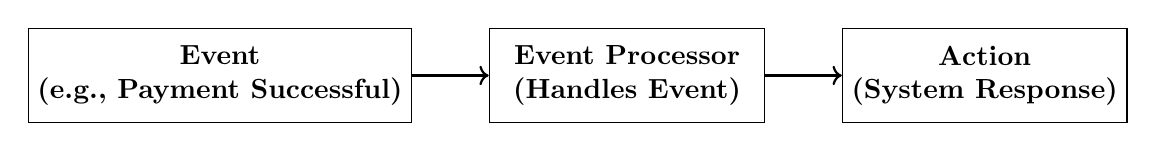
\begin{tikzpicture}[
			node distance=0.08\textwidth,
			every node/.style={draw, align=center, minimum height=1.2cm, minimum width=3.5cm, font=\bfseries},
			arrow/.style={->, thick}
			]
			% Nodes
			\node (event) {Event \\ (e.g., Payment Successful)};
			\node (processor) [right=of event] {Event Processor \\ (Handles Event)};
			\node (action) [right=of processor] {Action \\ (System Response)};
			
			% Arrows
			\draw[arrow] (event) -- (processor);
			\draw[arrow] (processor) -- (action);
		\end{tikzpicture}
		
		\vspace{10pt}
		\scriptsize \textit{Simple event processed immediately into an action.}
		
		\vspace{15pt}
		\begin{columns}[T]
			\column{0.5\textwidth}
			\textbf{Overview and Examples:}
			\begin{itemize}
				\item Basic form of EDA
				\item One event → one immediate action
				\item No event correlation needed
				\item Examples:
				\begin{itemize}
					\item Payment success → Issue invoice
					\item High temperature → Trigger alarm
				\end{itemize}
			\end{itemize}
			
			\column{0.5\textwidth}
			\textbf{Common Uses and Benefits:}
			\begin{itemize}
				\item Monitoring systems
				\item Notification services
				\item Simple triggered workflows
				\item Benefits:
				\begin{itemize}
					\item Fast, predictable responses
					\item Easy to design and scale
				\end{itemize}
			\end{itemize}
		\end{columns}
	\end{frame}
	
	\subsection{Complex Event Processing in EDA}
	\begin{frame}[fragile]{Complex Event Processing in EDA}
		\vspace{20pt}
		\centering
		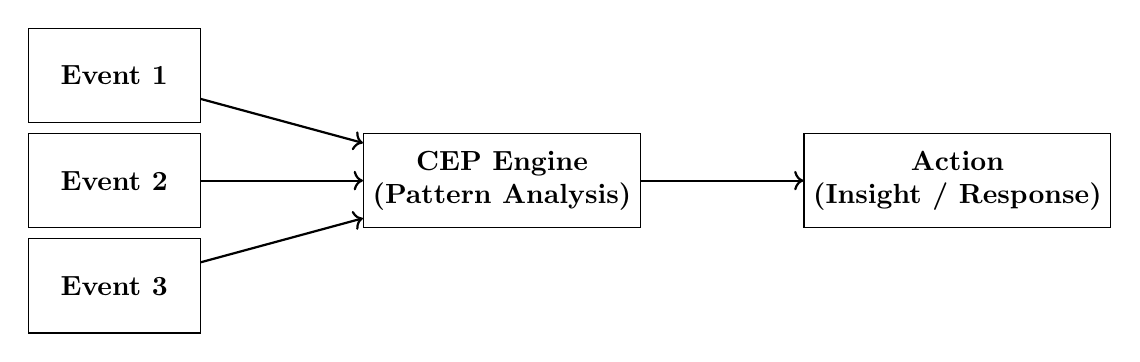
\begin{tikzpicture}[
			node distance=0.01\textwidth and 0.07\textwidth,
			every node/.style={draw, align=center, minimum height=1.2cm, minimum width=0.18\textwidth, font=\bfseries},
			arrow/.style={->, thick}
			]
			% Nodes
			\node (event1) {Event 1};
			\node (event2) [below=of event1] {Event 2};
			\node (event3) [below=of event2] {Event 3};
			\node (engine) [right=of event2, xshift=0.1\textwidth] {CEP Engine \\ (Pattern Analysis)};
			\node (action) [right=of engine, xshift=0.1\textwidth] {Action \\ (Insight / Response)};
			
			% Arrows
			\draw[arrow] (event1) -- (engine);
			\draw[arrow] (event2) -- (engine);
			\draw[arrow] (event3) -- (engine);
			\draw[arrow] (engine) -- (action);
		\end{tikzpicture}
		
		\begin{columns}[T]
			\column{0.5\textwidth}
			\textbf{Overview:}
			\begin{itemize}
				\item Analyse multiple events over time
				\item Detect patterns, anomalies, sequences
				\item Find insights beyond single events
			\end{itemize}
			
			\column{0.5\textwidth}
			\textbf{Examples and Uses:}
			\begin{itemize}
				\item Fraud detection
				\item Network intrusion monitoring
				\item Stream filtering, matching, windowing
			\end{itemize}
		\end{columns}
		
	\end{frame}
	
	\subsection{Event Stream Processing in EDA}
	\begin{frame}[fragile]{Event Stream Processing in EDA}
		\vspace{20pt}
		\centering
		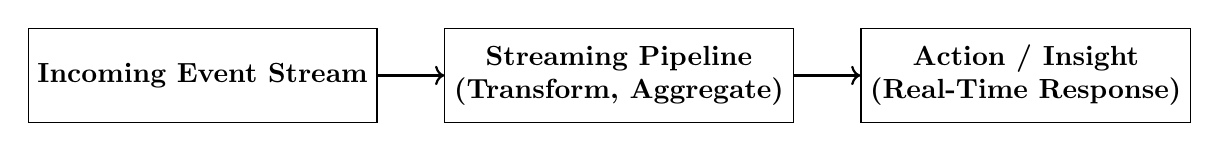
\begin{tikzpicture}[
			node distance=0.07\textwidth,
			every node/.style={draw, align=center, minimum height=1.2cm, minimum width=3.5cm, font=\bfseries},
			arrow/.style={->, thick}
			]
			% Nodes
			\node (stream) {Incoming Event Stream};
			\node (pipeline) [right=of stream] {Streaming Pipeline \\ (Transform, Aggregate)};
			\node (output) [right=of pipeline] {Action / Insight \\ (Real-Time Response)};
			
			% Arrows
			\draw[arrow] (stream) -- (pipeline);
			\draw[arrow] (pipeline) -- (output);
		\end{tikzpicture}
		
		\vspace{10pt}
		\scriptsize \textit{Streaming events processed continuously through a pipeline to generate real-time actions or insights.}
		
		\vspace{15pt}
		\begin{columns}[T]
			\column{0.5\textwidth}
			\textbf{Overview:}
			\begin{itemize}
				\item Real-time continuous event processing
				\item Supports transformation, aggregation, enrichment
				\item Focus on low-latency and high-throughput
			\end{itemize}
			
			\column{0.5\textwidth}
			\textbf{Examples and Platforms:}
			\begin{itemize}
				\item Real-time social media analytics
				\item IoT sensor monitoring
				\item User behaviour-based recommendations
				\item Platforms: Kafka, Flink, Spark Streaming
			\end{itemize}
		\end{columns}
	\end{frame}
	
	\section{Implementation Patterns of EDA}
	
	\begin{frame}{\hfill}
		\centering
		\Huge \textbf{Implementation Patterns of Event-Driven Architecture}
	\end{frame}
	
	\subsection{Publish/Subscribe}
	
	\begin{frame}[fragile]{Publish/Subscribe Pattern in EDA}
		\vspace{20pt}
		\centering
		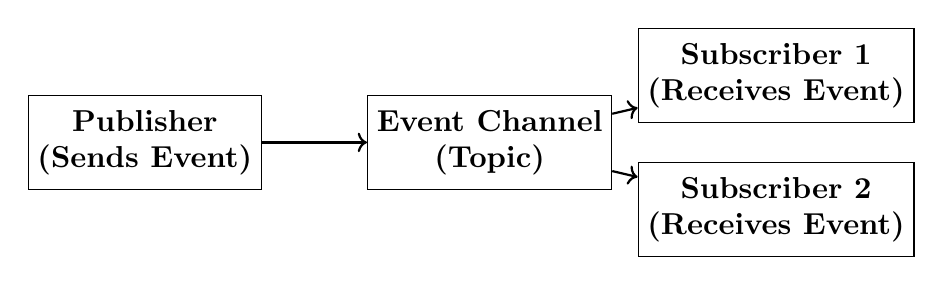
\begin{tikzpicture}[
			node distance=-0.02\textwidth and 0.06\textwidth,
			every node/.style={draw, align=center, minimum height=1.2cm, minimum width=0.13\textwidth, font=\fontsize{11}{13}\selectfont\bfseries},
			arrow/.style={->, thick}
			]
			% Nodes
			\node (publisher) {Publisher \\ (Sends Event)};
			\node (channel) [right=of publisher, xshift=0.05\textwidth] {Event Channel \\ (Topic)};
			\node (subscriber1) [above=of channel, xshift=0.3\textwidth, yshift=-0.01\textwidth] {Subscriber 1 \\ (Receives Event)};
			\node (subscriber2) [below=of channel, xshift=0.3\textwidth, yshift=0.01\textwidth] {Subscriber 2 \\ (Receives Event)};
			
			% Arrows
			\draw[arrow] (publisher) -- (channel);
			\draw[arrow] (channel) -- (subscriber1);
			\draw[arrow] (channel) -- (subscriber2);
		\end{tikzpicture}
		\vfill
		\begin{columns}[T]
			\column{0.5\textwidth}
			\textbf{Overview:}
			\begin{itemize}
				\item Basic communication pattern in EDA
				\item Publisher and subscriber are loosely coupled
				\item Supports asynchronous, many-to-many communication
			\end{itemize}
			
			\column{0.5\textwidth}
			\textbf{Examples and Platforms:}
			\begin{itemize}
				\item Message brokers: Kafka, RabbitMQ, Redis Pub/Sub
				\item Scalable and flexible event delivery
				\item Independent evolution of components
			\end{itemize}
		\end{columns}
	\end{frame}
	
	\subsection{Event Sourcing}
	
	\begin{frame}[fragile]{Event Sourcing Pattern in EDA}
		\vspace{20pt}
		\centering
		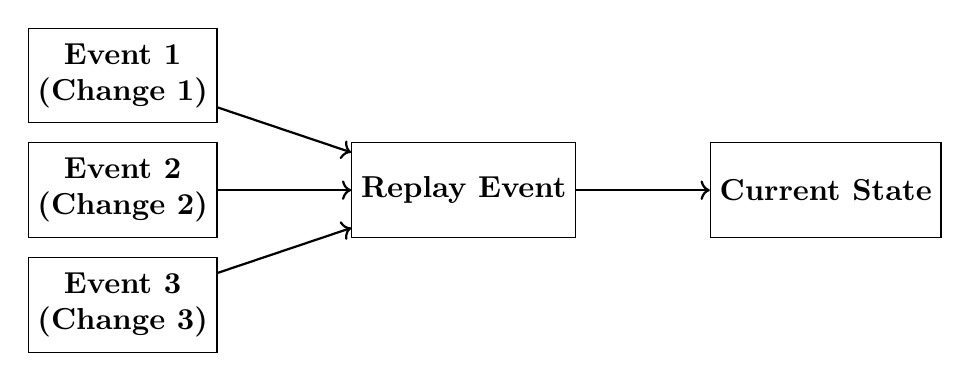
\begin{tikzpicture}[
			node distance=0.02\textwidth and 0.06\textwidth,
			every node/.style={draw, align=center, minimum height=1.2cm, minimum width=0.13\textwidth, font=\fontsize{11}{13}\selectfont\bfseries},
			arrow/.style={->, thick}
			]
			% Nodes
			\node (event1) {Event 1 \\ (Change 1)};
			\node (event2) [below=of event1] {Event 2 \\ (Change 2)};
			\node (event3) [below=of event2] {Event 3 \\ (Change 3)};
			\node (replay) [right=of event2, xshift=0.08\textwidth] {Replay Event};
			\node (current) [right=of replay, xshift=0.08\textwidth] {Current State};
			
			% Arrows
			\draw[arrow] (event1) -- (replay);
			\draw[arrow] (event2) -- (replay);
			\draw[arrow] (event3) -- (replay);
			\draw[arrow] (replay) -- (current);
		\end{tikzpicture}
		
		\scriptsize \textit{System state is built by replaying the full historical sequence of events.}
		
		\begin{columns}[T]
			\column{0.5\textwidth}
			\textbf{Overview:}
			\begin{itemize}
				\item Stores all state changes as events
				\item Rebuilds current state by replaying events
				\item Enhances transparency, auditability, resilience
			\end{itemize}
			
			\column{0.5\textwidth}
			\textbf{Challenges and Uses:}
			\begin{itemize}
				\item Requires careful event schema design
				\item Needs versioning and data volume management
				\item Common in systems needing event replay or historical trace
			\end{itemize}
		\end{columns}
	\end{frame}
	
	\subsection{CQRS (Command Query Responsibility Segregation)}
	
	\begin{frame}[fragile]{CQRS Pattern in EDA}
		\vspace{20pt}
		\centering
		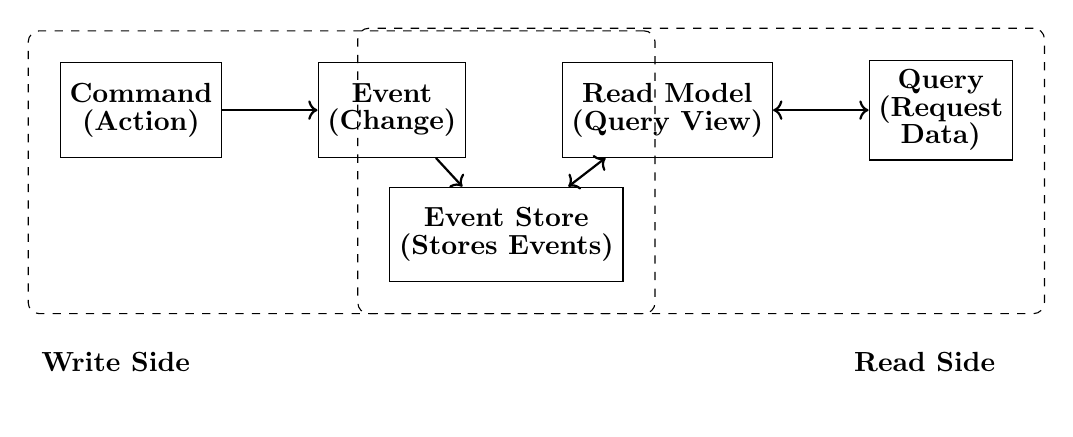
\begin{tikzpicture}[
			node distance=0.01\textwidth and 0.02\textwidth,
			every node/.style={draw, align=center, minimum height=1.2cm, minimum width=0.13\textwidth, font=\fontsize{10}{10}\selectfont\bfseries},
			group/.style={draw, dashed, inner sep=0.4cm, rounded corners},
			arrow/.style={->, thick},
			bidir/.style={<->, thick}
			]
			% Nodes
			\node (command) {Command \\ (Action)};
			\node (event) [right=of command, xshift=0.08\textwidth] {Event \\ (Change)};
			\node (store) [below=of event, xshift=0.12\textwidth, yshift=-0.02\textwidth] {Event Store \\ (Stores Events)};
			\node (readmodel) [right=of event, xshift=0.08\textwidth] {Read Model \\ (Query View)};
			\node (query) [right=of readmodel, xshift=0.08\textwidth] {Query \\ (Request \\ Data)};
			
			% Groupings
			\node[group, fit=(command) (event) (store), label=below left:{\textbf{Write Side}}] (writegroup) {};
			\node[group, fit=(store) (readmodel) (query), label=below right:{\textbf{Read Side}}] (readgroup) {};
			
			% Arrows
			\draw[arrow] (command) -- (event);
			\draw[arrow] (event) -- (store);
			\draw[bidir] (store) -- (readmodel);
			\draw[bidir] (readmodel) -- (query);
		\end{tikzpicture}
	\vspace{-20pt}
	\begin{columns}[T]
		\column{0.45\textwidth}
		\textbf{Overview:}
		\begin{itemize}
			\item Split writes and reads
			\item Optimise each side separately
			\item Common in EDA systems
		\end{itemize}
		
		\column{0.55\textwidth}
		\textbf{Benefits and Challenges:}
		\begin{itemize}
			\item Improves scalability and domain clarity
			\item Needs careful event and version design
			\item Adds complexity; use when necessary
		\end{itemize}
	\end{columns}
	
	\end{frame}
	
	
	\section{Best Practices}

	\begin{frame}[fragile]{Best Practices in EDA}
		\vspace{20pt}
		\begin{columns}[T]
			\column{0.33\textwidth}
			\textbf{Good Event Design:}
			\begin{itemize}
				\item Events represent meaningful changes
				\item Use clear action-based names (e.g., OrderCreated)
				\item Payloads should be explicit, minimal, and evolvable
				\item Ensure backward compatibility
			\end{itemize}
			
			\column{0.33\textwidth}
			\textbf{Error Handling and Retry:}
			\begin{itemize}
				\item Distinguish transient vs permanent errors
				\item Retry with backoff for transient issues
				\item Use Dead Letter Queues (DLQ) for permanent errors
				\item Design idempotent event handlers
			\end{itemize}
			
			\column{0.33\textwidth}
			\textbf{Observability and Monitoring:}
			\begin{itemize}
				\item Log event metadata (ID, timestamp, status)
				\item Collect metrics (latency, failure rate, queue size)
				\item Implement distributed tracing
				\item Enable faster diagnosis and recovery
			\end{itemize}
		\end{columns}
	\end{frame}
	
	
\section{Simple Kafka-Based EDA Implementation}

\begin{frame}[fragile]{Simple Kafka-Based EDA Architecture}
	\vspace{20pt}
	\centering
	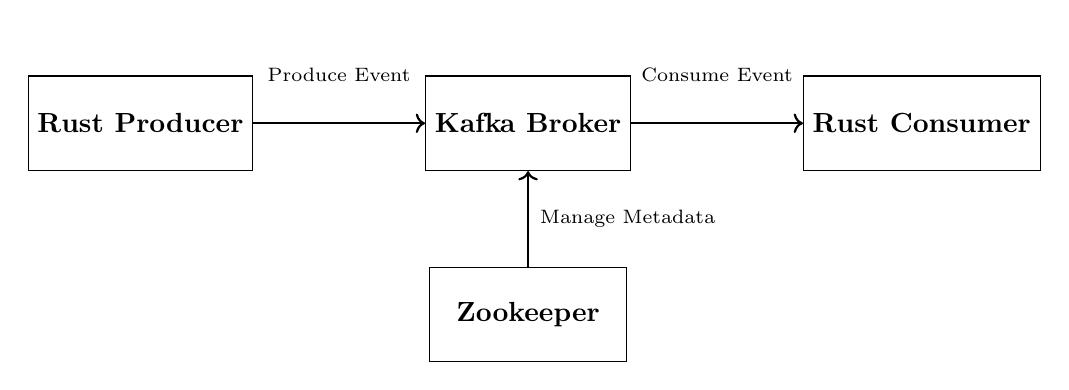
\begin{tikzpicture}[
		node distance=0.06\textwidth and 0.08\textwidth,
		every node/.style={draw, align=center, minimum height=1.2cm, minimum width=2.5cm, font=\bfseries},
		arrow/.style={->, thick}
		]
		% Nodes
		\node (producer) {Rust Producer};
		\node (kafka) [right=of producer, xshift=0.1\textwidth] {Kafka Broker};
		\node (consumer) [right=of kafka, xshift=0.1\textwidth] {Rust Consumer};
		\node (zookeeper) [below=of kafka, yshift=-0.04\textwidth] {Zookeeper};
		
		% Arrows with pure text labels (no node)
		\draw[arrow] (producer) -- node[midway, above, font=\scriptsize, draw=none] {Produce Event} (kafka);
		\draw[arrow] (kafka) -- node[midway, above, font=\scriptsize, draw=none] {Consume Event} (consumer);
		\draw[arrow] (zookeeper) -- node[midway, right, font=\scriptsize, draw=none] {Manage Metadata} (kafka);
	\end{tikzpicture}
	
	\scriptsize \textit{Producer sends events to Kafka; Kafka delivers to Consumer; Zookeeper manages cluster coordination.}
\end{frame}

	
	
	\begin{frame}[fragile]{Conclusion}
		\vspace{20pt}
		\begin{columns}[T]
			\column{0.33\textwidth}
			\textbf{Core Concepts:}
			\begin{itemize}
				\item Event is the primary unit of communication
				\item Event Producer, Event Consumer, Event Bus
				\item Enables responsive, scalable, flexible systems
			\end{itemize}
			
			\column{0.33\textwidth}
			\textbf{Implementation Patterns:}
			\begin{itemize}
				\item Publish/Subscribe: loose coupling communication
				\item Event Sourcing: full audit and state reconstruction
				\item CQRS: optimised command and query separation
			\end{itemize}
			
			\column{0.33\textwidth}
			\textbf{Challenges and Best Practices:}
			\begin{itemize}
				\item Handle debugging, consistency, infrastructure complexity
				\item Design clear and evolvable events
				\item Apply observability and reliable error handling
			\end{itemize}
		\end{columns}
	\end{frame}
	
\end{document}
